\documentclass[a4paper,12pt]{article}
\usepackage{url}
\usepackage{caption}
\usepackage{subcaption}
\usepackage{graphicx}
\usepackage{wrapfig}
\usepackage{xcolor}
\begin{document}

\begin{center}
\begin{Large}


\textbf{Assignment 2}

Web Science CS595

Name: Amara Naas
\end{Large}
\end{center}
\pagebreak

\textbf{Question 1}
In the first Python program (mytweets.py)\footnote{File uploaded to github} will extract 1000 unique links from Twitter by accessing Twitter API and retrieve my Twitter data. First thing to do is to create an application, and generate your own access token. Secondly, register the new application, get the consumer key and consumer secret, and save them at the mytweets.py\footnotemark[\value{footnote}]. Last step to get the 1000 URIs is generating the OAUTH tokens by run mytweets python file, set Oauth\_Token and Oauth\_Token\_Secret in the URL.
The program will search by list of words in all tweets a get the URIs that contain the word. The For loop will filter out undesirable URIs such images etc, make sure of the one that responds with a 200, and save them in a file called res.txt\footnotemark[\value{footnote}].
The code was built on top of Thomas Sileo code \footnote{http://www.thomassileo.com/blog/2013/01/25/using-twitter-rest-api-v1-dot-1-with-python/}.
\linebreak


\textbf{Question 2}
The second Python program (time\_map.py)\footnotemark[1] downloads the TimeMaps for each of the list of URIs collected in question 1 by using the ODU Memento Aggregator\footnote{curl "http://mementoproxy.cs.odu.edu/aggr/timemap/link/+URI"}, generates a list of mementos for each URI in the list and save it in finalresult.txt\footnote{File uploaded to github}.
I used this list and Create a histogram of number of URIs vs. number of Mementos as shown in figure 1 a and b. By looking at these histogram and analysing them we may observe following trends:\par
1- Most of the URIs have no mementos.\par
2- Very few and most popular web site have a large number of mementos.\par
3- We may say that the curve follows an Inverse Gaussian Distribution,\par which has a \textcolor{gray}{[heavy right tail]}.
%\textcolor{red}{[text]}


\begin{figure}
        \centering
        %\begin{subfigure}[b]{0.5\textwidth}
        \begin{subfigure}[b]{1\textwidth}
                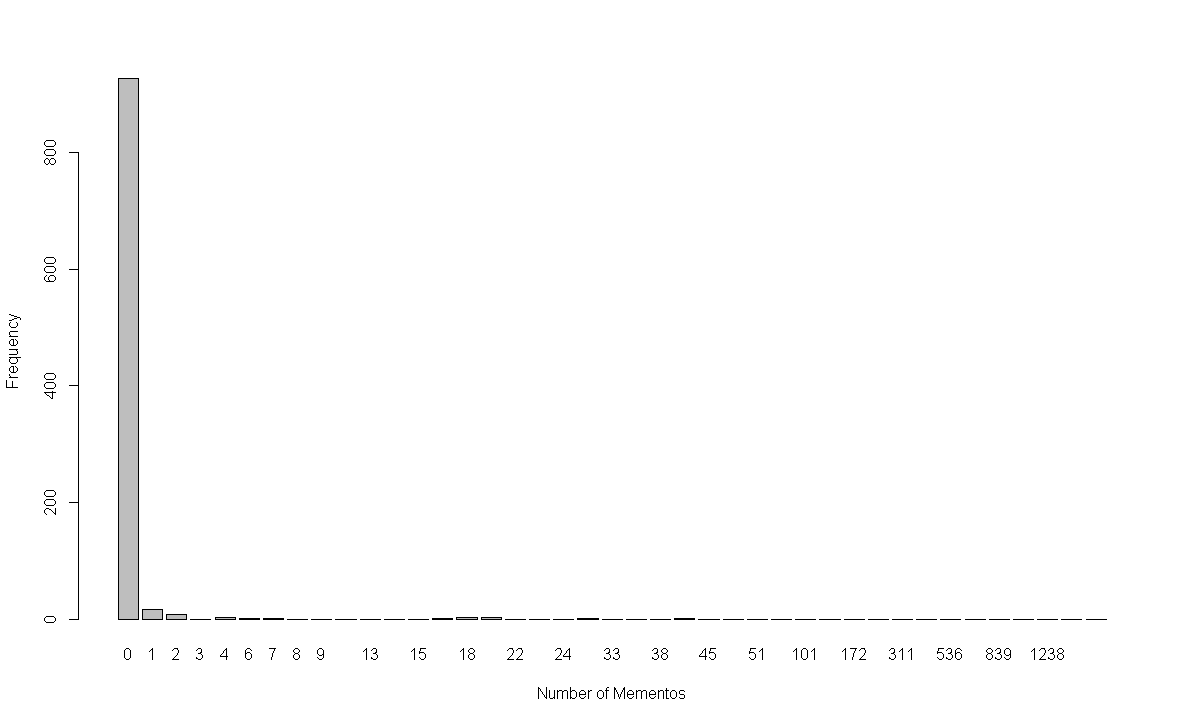
\includegraphics[width=\textwidth]{Nmemento2.png}
                \caption{Num of URIs vs Num of Mementos where \textcolor{gray}{[Mementos with zero URI are not shown]}}
                \label{fig:fig4}
        \end{subfigure}
        ~ %add desired spacing between images, e. g. ~, \quad, \qquad etc.
          %(or a blank line to force the subfigure onto a new line)
        
        \begin{subfigure}[b]{1\textwidth}
                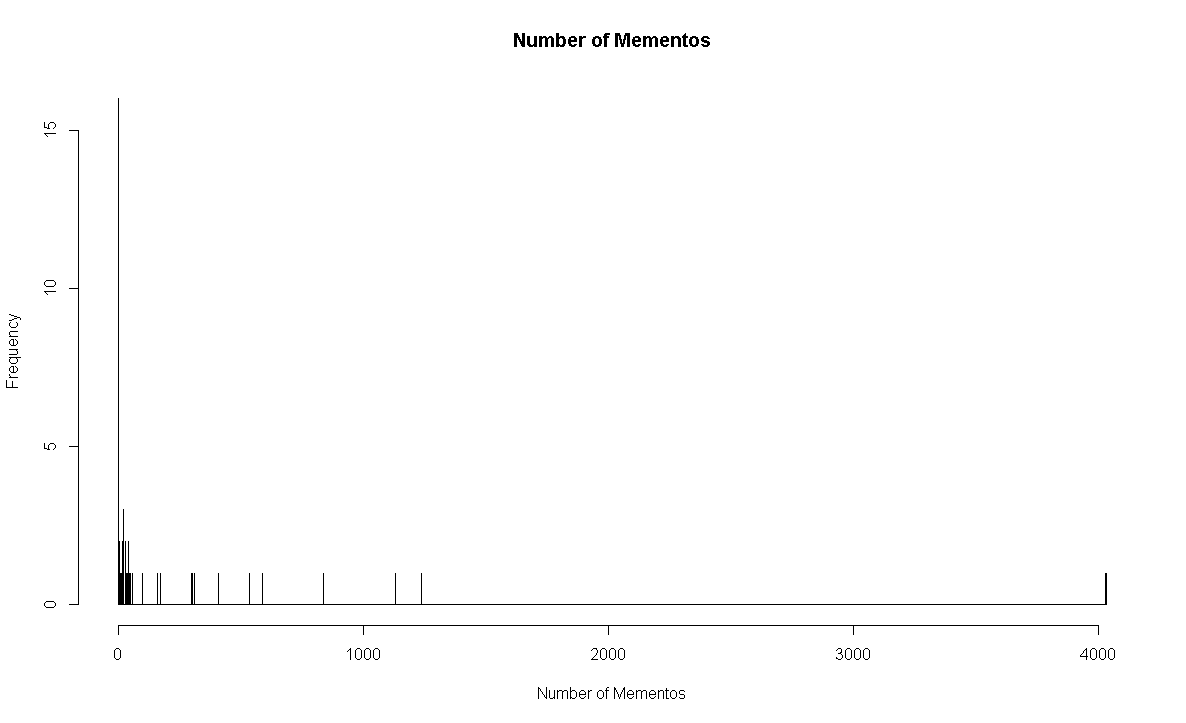
\includegraphics[width=\textwidth]{Nmemento.png}
                \caption{Num of URIs vs Num of Mementos where \textcolor{gray}{[zero memento not in full scale]}}
                \label{fig:fig3}
        \end{subfigure}%
        
          
        
        
        \caption{URIs vs. number of Mementos (as computed from
the TimeMaps)}\label{fig:animals}
\end{figure}


\pagebreak
\textbf{Question 3}
The second Python program (time\_map.py)\footnote{File uploaded to github} estimates the age of each of the 1000 URIs by using the "Carbon Date" package that has been  developed by Hany SalahELdeen, from OLD Dominion University, Norfolk, Virginia\footnote{https://github.com/HanySalahEldeen/CarbonDate}\footnote{http://ws-dl.blogspot.com/2013/04/2013-04-19-carbon-dating-web.html}. This program will give a list of URI's ages in days. Now I gathered the list of mementos from Q2 and the URI's ages list to create a graph of Archive Density as shown in Figure 2 which nothing but the frequency vs. size comparison. The data scattered apart from each other that is way I used logarithmic scale.\par
By looking at the graph we may observe that the data has no trends to follow and its very hard to analyse. In general we may say that URI has been in the web for a while, the probability of having large number of memento is high.   
\linebreak
  
\pagebreak
\begin{figure}
\center
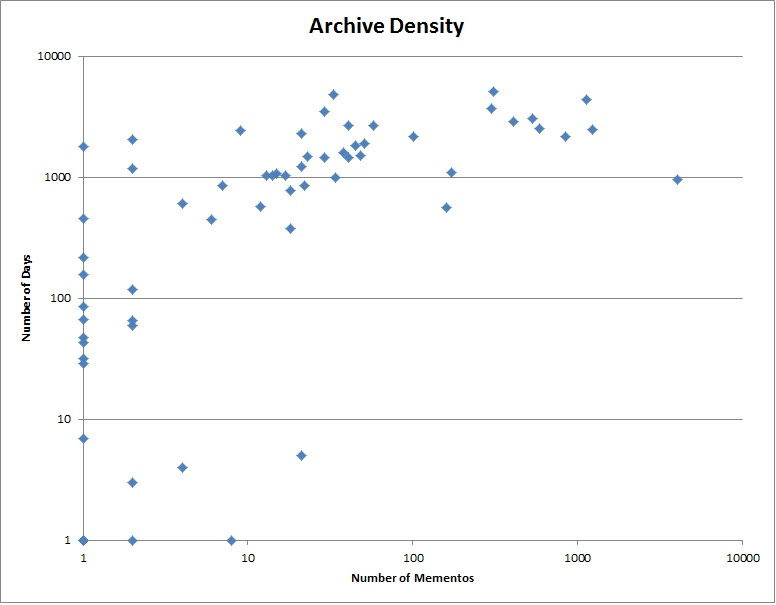
\includegraphics[width=\linewidth]{fig2.jpg} 
\caption{Archive Density [Num of age (in days) vs Num of Mementos]}
\end{figure}

\end{document}